% ------------------------------------------------------------------------------
% TYPO3 CMS 8.0 - What's New - Chapter "Introduction" (English Version)
%
% @author	Michael Schams <schams.net>
% @license	Creative Commons BY-NC-SA 3.0
% @link		http://typo3.org/download/release-notes/whats-new/
% @language	English
% ------------------------------------------------------------------------------
% LTXE-CHAPTER-UID:		cb43d098-7bf9a537-bf3817c0-53a0f29f
% LTXE-CHAPTER-NAME:	Introduction
% ------------------------------------------------------------------------------

\section{Inleiding}
\begin{frame}[fragile]
	\frametitle{Inleiding}

	\begin{center}\huge{Inleiding}\end{center}
	\begin{center}\huge{\color{typo3darkgrey}\textbf{De feiten}}\end{center}

\end{frame}

% ------------------------------------------------------------------------------
% LTXE-SLIDE-START
% LTXE-SLIDE-UID:		130a7731-2873d2c3-f3379d30-6cb3d12f
% LTXE-SLIDE-ORIGIN:	9e397afb-762f7061-0e0e0bd1-9836250e English
% LTXE-SLIDE-TITLE:		TYPO3 CMS 8.0 - The Facts
% ------------------------------------------------------------------------------
\begin{frame}[fragile]
	\frametitle{Inleiding}
	\framesubtitle{TYPO3 CMS 8.0 - De feiten}

	\begin{itemize}
		\item Publicatiedatum: 22 maart 2016
		\item Publicatietype: Sprint Release
		\item Slogan: Start de motoren
	\end{itemize}

	\begin{figure}
		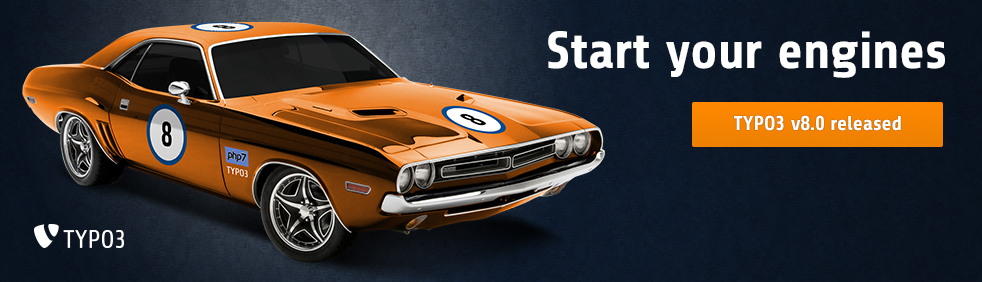
\includegraphics[width=0.95\linewidth]{Introduction/typo3cms80-banner.png}
	\end{figure}

\end{frame}

% ------------------------------------------------------------------------------
% LTXE-SLIDE-START
% LTXE-SLIDE-UID:		23dbb2d0-296e82e4-ed80e11f-e4eaab7a
% LTXE-SLIDE-ORIGIN:	737c8e9b-4ae60e26-6975ea72-21146dd0 English
% LTXE-SLIDE-TITLE:		System Requirements
% ------------------------------------------------------------------------------
\begin{frame}[fragile]
	\frametitle{Inleiding}
	\framesubtitle{Systeemeisen}

	\begin{itemize}
		\item PHP:\tabto{2.2cm}versie 7
		\item MySQL:\tabto{2.2cm}versie 5.5 tot 5.7
		\item Schijfruimte:\tabto{2.2cm}min 200 MB
		\item PHP-instellingen:

			\begin{itemize}
				\item \texttt{memory\_limit} >= 128M
				\item \texttt{max\_execution\_time} >= 240s
				\item \texttt{max\_input\_vars} >= 1500
				\item compilatieoptie \texttt{-}\texttt{-disable-ipv6} mag \underline{niet} gebruikt worden
			\end{itemize}

		\item De backend vereist Microsoft Internet Explorer 11 of later,
			Microsoft Edge, Google Chrome, Firefox, Safari of een andere moderne
			compatibele browser

	\end{itemize}

\end{frame}

% ------------------------------------------------------------------------------
% LTXE-SLIDE-START
% LTXE-SLIDE-UID:		ab638613-cce01ca3-79503915-8c86a0b6
% LTXE-SLIDE-ORIGIN:	90d2d3d1-f9d57661-dd01143b-10630416 English
% LTXE-SLIDE-TITLE:		Development And Release Timeline
% ------------------------------------------------------------------------------
\begin{frame}[fragile]
	\frametitle{Inleiding}
	\framesubtitle{Planning voor ontwikkeling en publicatie}

	\begin{figure}
		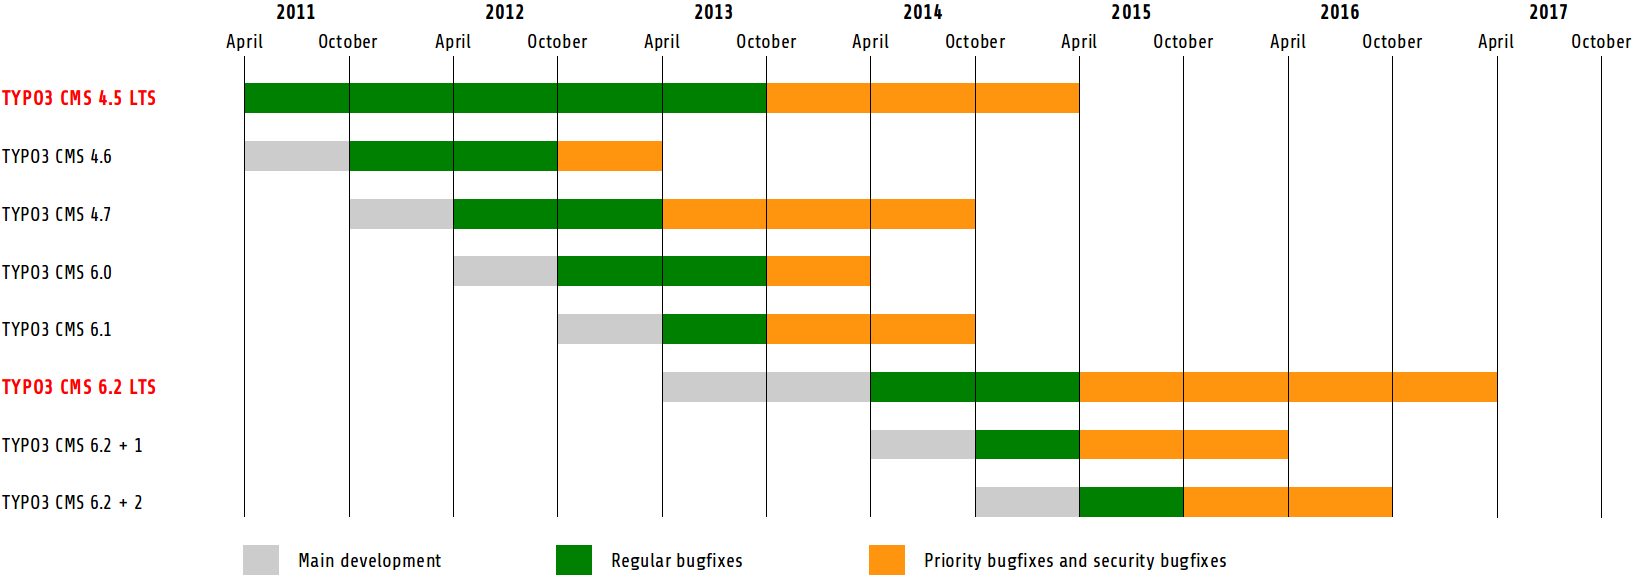
\includegraphics[width=1\linewidth]{Introduction/ReleaseAgenda.png}
	\end{figure}

\end{frame}

% ------------------------------------------------------------------------------
% LTXE-SLIDE-START
% LTXE-SLIDE-UID:		56815476-edd38787-4f79d00d-58db0804
% LTXE-SLIDE-ORIGIN:	13e0fd6a-fa50d02d-c15c4af0-f3996926 English
% LTXE-SLIDE-TITLE:		TYPO3 CMS Roadmap
% ------------------------------------------------------------------------------
\begin{frame}[fragile]
	\frametitle{Inleiding}
	\framesubtitle{TYPO3 CMS Roadmap}

	Publicatiedatums en primaire focus:

	\begin{itemize}

		\item
			\begingroup
				\color{typo3orange}
					v8.0 \tabto{1.1cm}22/Mar/2016\tabto{3.4cm}Last minute toevoegingen
			\endgroup
		\item v8.1 \tabto{1.1cm}03 mei 2016\tabto{3.4cm}Cloud-itegratie
		\item v8.2 \tabto{1.1cm}05 jul 2016\tabto{3.4cm}Rich Text Editor
		\item v8.3 \tabto{1.1cm}30 aug 2016\tabto{3.4cm}Bewerken in Frontend powereditie
		\item v8.4 \tabto{1.1cm}18 okt 2016\tabto{3.4cm}\textit{onbekend}
		\item v8.5 \tabto{1.1cm}20 dec 2016\tabto{3.4cm}Integrator-ondersteuning
		\item v8.6 \tabto{1.1cm}14 feb 2017\tabto{3.4cm}\textit{onbekend}
		\item v8.7 \tabto{1.1cm}04 apr 2017\tabto{3.4cm}LTS Voorbereiding

	\end{itemize}

	\smaller
		\url{https://typo3.org/typo3-cms/roadmap/}\newline
		\url{https://typo3.org/news/article/kicking-off-typo3-v8-development/}
	\normalsize

\end{frame}

% ------------------------------------------------------------------------------
% LTXE-SLIDE-START
% LTXE-SLIDE-UID:		abbf3511-e60c8b6e-f01361ba-daf09507
% LTXE-SLIDE-ORIGIN:	06c6100a-69216610-618bde63-bbdc4eef English
% LTXE-SLIDE-TITLE:		Installation
% ------------------------------------------------------------------------------
\begin{frame}[fragile]
	\frametitle{Inleiding}
	\framesubtitle{Installatie}

	\begin{itemize}
		\item Officiële installatieprocedure op Linux/Mac OS X\newline
			(DocumentRoot bijvoorbeeld \texttt{/var/www/site/htdocs}):
		\begin{lstlisting}
			$ cd /var/www/site
			$ wget --content-disposition get.typo3.org/8.0
			$ tar xzf typo3_src-8.0.0.tar.gz
			$ cd htdocs
			$ ln -s ../typo3_src-8.0.0 typo3_src
			$ ln -s typo3_src/index.php
			$ ln -s typo3_src/typo3
			$ touch FIRST_INSTALL
		\end{lstlisting}

		\item Symbolische links op Microsoft Windows:

			\begin{itemize}
				\item Gebruik \texttt{junction} op Windows XP/2000
				\item Gebruik \texttt{mklink} op Windows Vista en Windows 7
			\end{itemize}

	\end{itemize}
\end{frame}

% ------------------------------------------------------------------------------
% LTXE-SLIDE-START
% LTXE-SLIDE-UID:		220eb84a-2d82009c-f0c5382c-0316dbf9
% LTXE-SLIDE-ORIGIN:	b878899c-e4b09ddf-4c0ea575-9e0900ad English
% LTXE-SLIDE-TITLE:		Upgrade to TYPO3 CMS 7
% ------------------------------------------------------------------------------
\begin{frame}[fragile]
	\frametitle{Inleiding}
	\framesubtitle{Upgrade naar TYPO3 CMS 8.x}

	\begin{itemize}
		\item Upgrades alleen mogelijk vanaf TYPO3 CMS 7.6 LTS
		\item TYPO3 CMS < 7.6 LTS moet eerst naar TYPO3 CMS 7.6 LTS bijgewerkt worden
	\end{itemize}

	\begin{itemize}

		\item Upgrade-instructies:\newline
			\smaller\url{http://wiki.typo3.org/Upgrade#Upgrading_to_8.0}\normalsize
		\item Officiële TYPO3-handleiding "TYPO3 Installation and Upgrading":
			\smaller\url{http://docs.typo3.org/typo3cms/InstallationGuide}\normalsize
		\item Algemene aanpak:
			\begin{itemize}
				\item Controleer minimale systeemeisen \small(PHP, MySQL, etc.)
				\item Bekijk \textbf{deprecation\_*.log} in oude TYPO3 installatie
				\item Update alle extensies naar laatste versie
				\item Zet nieuwe broncode neer en start Install Tool -> Upgrade Wizard
				\item Bekijk startmodule voor backend gebruikers (optioneel)
			\end{itemize}
	\end{itemize}

\end{frame}

% ------------------------------------------------------------------------------

% ------------------------------------------------------------------------------
% LTXE-SLIDE-START
% LTXE-SLIDE-UID:		ff6dfa40-4f2581e1-a025e886-6d47ba46
% LTXE-SLIDE-ORIGIN:	e4b09ddf-4c0ea575-9e0900ad-b878899c English
% LTXE-SLIDE-TITLE:		PHP Version 7
% ------------------------------------------------------------------------------
\begin{frame}[fragile]
	\frametitle{Inleiding}
	\framesubtitle{PHP Versie 7}

	\begin{itemize}

		\item PHP 7.0 is de minimale eis voor TYPO3 CMS 8.x
		\item TYPO3 zal volgende PHP 7 versies ondersteunen wanneer deze uitkomen
		\item Deze versie geeft significant meer prestaties op het hele systeem

		\item Niet alleen backendgebruikers merken een soepelere interface, maar ook het
			nieuwe record voor een volledig gecachete pagina in de frontend is nu minder
			dan 7 milliseconde, wat ongeveer 40\% sneller is in vergelijking met dezelfde
			website met PHP versie 5.5

		\item We zijn ook begonnen nieuwe features van deze PHP-versie te gebruiken, bijvoorbeeld
			de cryptografisch veilige pseudo-random generatoren worden al ingezet

	\end{itemize}

\end{frame}

% ------------------------------------------------------------------------------
